\chapter{Results}

\section{Characteristics of the Respondents}
A total of 231 female students took part. Their mean age was $22.52\pm1.51$ years (range 18--28), and 95 (41.1\%) studied healthcare subjects while 136 (58.9\%) studied other subjects (Table~\ref{tab:sociodemo}). Three quarters (173 of 230, 75.2\%) reported that at least one parent had university-level education. Just over half (126, 54.5\%) had received some education on sexually transmitted infections, mostly through a formal class or curriculum (95 students).

A total of 182 of 228 students (79.8\%) had heard of HPV before the survey. This was more common among healthcare students than among others (90.5\% against 72.2\%, $p<0.001$). Self-rated knowledge was modest: 89 students (39.0\% of 228 who answered) rated it as poor and 13 (5.7\%) as none, while only 45 (19.7\%) rated it as good or excellent.

Talking about HPV was widely seen as taboo: 76 students (33.0\%) said ``yes, very much so'' and a further 83 (36.1\%) said ``somewhat''. Almost half (106, 45.9\%) said their parents had never discussed HPV or its vaccine with them. Only 92 (39.8\%) reported that their university had offered an HPV awareness programme, and 36 (15.6\%) were not aware of any.

\begin{longtable}{@{}>{\raggedright\arraybackslash}p{9.2cm}rr@{}}
\caption{Socio-demographic characteristics and background of the respondents ($N=231$).}\label{tab:sociodemo}\\
\toprule
Characteristic & $n$ & \% \\
\midrule
\endfirsthead
\caption[]{(continued)}\\
\toprule
Characteristic & $n$ & \% \\
\midrule
\endhead
\midrule\multicolumn{3}{r}{\emph{continued on next page}}\\
\endfoot
\bottomrule
\endlastfoot
\multicolumn{3}{l}{\textbf{Age (years)}} \\
\quad Mean $\pm$ SD & \multicolumn{2}{c}{22.52 $\pm$ 1.51} \\
\quad Median (range) & \multicolumn{2}{c}{23 (18--28)} \\
\quad 18--21 & 60 & 26.0 \\
\quad 22--23 & 105 & 45.5 \\
\quad 24 and above & 66 & 28.6 \\
\multicolumn{3}{l}{\textbf{Field of study}} \\
\quad Medical / Health sciences / Pharmacy / Nursing & 95 & 41.1 \\
\quad Engineering / Technology & 69 & 29.9 \\
\quad Arts / Humanities & 35 & 15.2 \\
\quad Science & 27 & 11.7 \\
\quad Commerce / Business & 2 & 0.9 \\
\quad Other & 3 & 1.3 \\
\multicolumn{3}{l}{\textbf{Academic stream (grouped)}} \\
\quad Healthcare & 95 & 41.1 \\
\quad Non-healthcare & 136 & 58.9 \\
\multicolumn{3}{l}{\textbf{Parents' highest education}} \\
\quad University / higher education & 173 & 74.9 \\
\quad Secondary school & 44 & 19.0 \\
\quad Primary school & 4 & 1.7 \\
\quad No formal education & 2 & 0.9 \\
\quad Not sure & 7 & 3.0 \\
\quad Missing & 1 & -- \\
\multicolumn{3}{l}{\textbf{Prior education/information on STIs}} \\
\quad Yes, formal class or curriculum & 95 & 41.1 \\
\quad Yes, through a health campaign & 31 & 13.4 \\
\quad No & 87 & 37.7 \\
\quad Not sure & 18 & 7.8 \\
\multicolumn{3}{l}{\textbf{Had heard of HPV before the survey}} \\
\quad Yes & 182 & 78.8 \\
\quad No & 46 & 19.9 \\
\quad Missing & 3 & -- \\
\multicolumn{3}{l}{\textbf{Parents/guardians discussed HPV or its vaccine}} \\
\quad Yes, in detail & 31 & 13.4 \\
\quad Briefly & 49 & 21.2 \\
\quad Never & 106 & 45.9 \\
\quad Not sure what they think & 45 & 19.5 \\
\multicolumn{3}{l}{\textbf{Discussing HPV considered taboo in own social context}} \\
\quad Yes, very much so & 76 & 32.9 \\
\quad Somewhat & 83 & 35.9 \\
\quad Not really & 54 & 23.4 \\
\quad No & 17 & 7.4 \\
\multicolumn{3}{l}{\textbf{University has provided an HPV vaccination awareness programme}} \\
\quad Yes & 92 & 39.8 \\
\quad No & 103 & 44.6 \\
\quad Not aware of any & 36 & 15.6 \\
\multicolumn{3}{l}{\textbf{Self-rated knowledge of HPV and its vaccine}} \\
\quad Excellent & 5 & 2.2 \\
\quad Good & 40 & 17.3 \\
\quad Moderate & 81 & 35.1 \\
\quad Poor & 89 & 38.5 \\
\quad None at all & 13 & 5.6 \\
\quad Missing & 3 & -- \\
\end{longtable}

\FloatBarrier

\section{Sources of Information About HPV}
Among the 182 students who had heard of HPV, the most common first source was the school or university curriculum (100, 54.9\%), followed by social media (56, 30.8\%) and family or friends (30, 16.5\%) (Figure~\ref{fig:sources}). Healthcare providers (17, 9.3\%), health campaigns (14, 7.7\%), newspapers (11, 6.0\%) and television or radio (8, 4.4\%) were much less common.

\begin{figure}[htbp]\centering
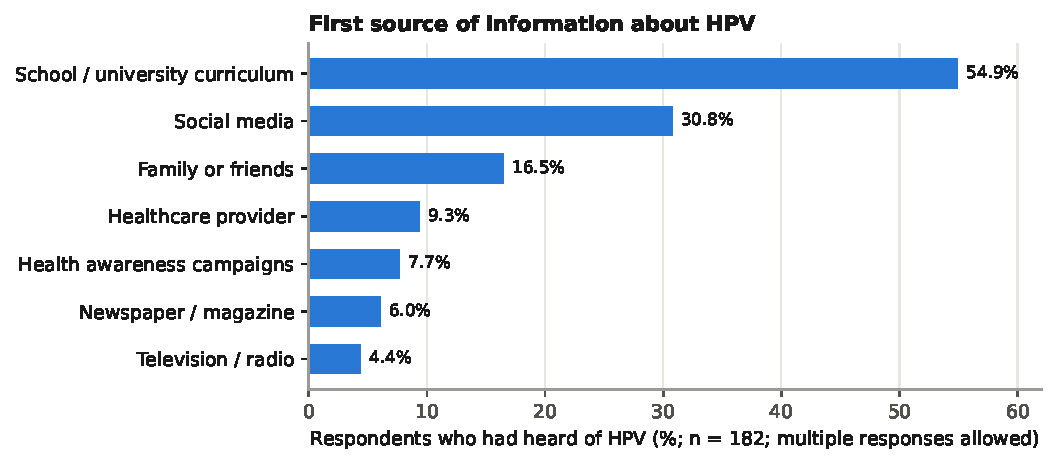
\includegraphics[width=.90\textwidth]{fig_sources}
\caption{First sources of information about HPV among students who had heard of it ($n=182$).}\label{fig:sources}
\end{figure}
\FloatBarrier

\section{Vaccination Status and Acceptance}
Only 18 students (7.8\%) had completed the vaccine course and 21 (9.1\%) had received some doses. Another 19 (8.2\%) were not sure, and 173 (74.9\%) had not been vaccinated. Among the 190 students who were unvaccinated or unsure and who answered the intention question, 75 (39.5\%) were ``likely'' and 70 (36.8\%) ``very likely'' to be vaccinated in future, 42 (22.1\%) were uncertain and 3 (1.6\%) were very unlikely.

Combining current vaccination with intention, 184 of 229 students (80.3\%) were classed as accepting HPV vaccination (Table~\ref{tab:acceptance}, Figure~\ref{fig:acceptance}). Acceptance was almost identical in healthcare students (75 of 94, 79.8\%) and non-healthcare students (109 of 135, 80.7\%; $p=0.99$).

\begin{table}[htbp]\centering\small
\caption{Vaccination status and intention to accept the HPV vaccine ($n=229$; two respondents who were unvaccinated did not answer the intention item).}\label{tab:acceptance}
\begin{tabularx}{\textwidth}{@{}>{\raggedright\arraybackslash}X rr@{}}\toprule
Category & $n$ & \% \\\midrule
Fully vaccinated (all doses completed) & 18 & 7.9 \\
Partially vaccinated & 21 & 9.2 \\
\midrule
Not vaccinated or unsure; "very likely" to accept & 70 & 30.6 \\
Not vaccinated or unsure; "likely" to accept & 75 & 32.8 \\
Not vaccinated or unsure; "uncertain" & 42 & 18.3 \\
Not vaccinated or unsure; "very unlikely" & 3 & 1.3 \\
\midrule
\textbf{Accepting} (vaccinated, or likely/very likely) & \textbf{184} & \textbf{80.3} \\
\textbf{Not accepting} (uncertain or very unlikely) & \textbf{45} & \textbf{19.7} \\
\bottomrule\end{tabularx}\end{table}

\FloatBarrier
\begin{figure}[htbp]\centering
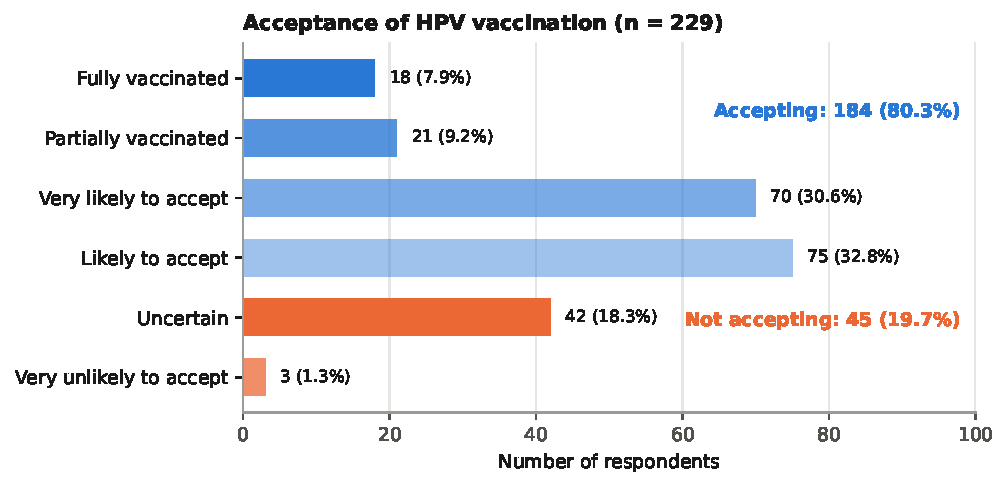
\includegraphics[width=.90\textwidth]{fig_acceptance}
\caption{Vaccination status and intention to be vaccinated ($n=229$).}\label{fig:acceptance}
\end{figure}
\FloatBarrier

\section{Knowledge of HPV}
The mean knowledge score was $6.32\pm3.67$ out of 15 (42.1\%; median 6, IQR 4.0--8.5). Most students had poor knowledge (155, 67.1\%); 55 (23.8\%) had moderate and 21 (9.1\%) good knowledge (Table~\ref{tab:scores}, Figure~\ref{fig:kdist}).

Healthcare students scored higher than non-healthcare students ($7.42\pm3.12$ against $5.54\pm3.84$; Mann--Whitney $U=8{,}421.5$, $p<0.001$). The share with poor knowledge was lower among healthcare students (61.1\% against 71.3\%), but the difference in knowledge categories was not statistically significant ($p=0.24$), and even among healthcare students only 11 (11.6\%) had good knowledge.

The best-answered statements were that the abbreviation HPV stands for human papillomavirus (78.8\% correct) and that HPV can lead to cervical cancer (78.4\%) (Table~\ref{tab:kitems}, Figure~\ref{fig:kitems}). Knowledge was weakest on the two false statements: only 9.5\% correctly rejected the claim that HPV causes menstrual problems and 13.0\% the claim that the vaccine protects against all HPV strains. Only 16.0\% knew that HPV infection often needs no treatment, 30.3\% knew that the vaccine works best before sexual activity begins, and 31.6\% knew that males can also benefit from the vaccine. ``Not sure'' was the most frequent answer on 7 of the 15 statements, for example in 61.0\% of responses on the timing of vaccination and 55.4\% on the claim that the vaccine protects against all strains.

\begin{table}[htbp]\centering\footnotesize\setlength{\tabcolsep}{4pt}
\caption{Knowledge and attitude scores of healthcare and non-healthcare students ($N=231$).}\label{tab:scores}
\begin{tabularx}{\textwidth}{@{}>{\raggedright\arraybackslash}X cccc@{}}\toprule
 & Healthcare & Non-healthcare & Overall & $p$ \\
 & ($n=95$) & ($n=136$) & ($N=231$) &  \\\midrule
\textbf{Knowledge score (0--15)} &&&& \\
\quad Mean $\pm$ SD & 7.42 $\pm$ 3.12 & 5.54 $\pm$ 3.84 & 6.32 $\pm$ 3.67 & $<$0.001\textsuperscript{a} \\
\quad Median (IQR) & 7.00 (6.00--9.00) & 5.00 (2.00--8.00) & 6.00 (4.00--8.50) & \\
\quad Poor (0--7) & 58 (61.1) & 97 (71.3) & 155 (67.1) & \\
\quad Moderate (8--11) & 26 (27.4) & 29 (21.3) & 55 (23.8) & \\
\quad Good (12--15) & 11 (11.6) & 10 (7.4) & 21 (9.1) & \\
\midrule
\textbf{Attitude score (10--50)} &&&& \\
\quad Mean $\pm$ SD & 45.56 $\pm$ 3.91 & 44.08 $\pm$ 4.77 & 44.69 $\pm$ 4.48 & 0.013\textsuperscript{a} \\
\quad Median (IQR) & 46.00 (44.00--48.00) & 45.00 (41.00--48.00) & 45.56 (42.00--48.00) & \\
\quad Positive (40--50) & 87 (91.6) & 117 (86.0) & 204 (88.3) & \\
\quad Neutral (30--39) & 8 (8.4) & 18 (13.2) & 26 (11.3) & \\
\quad Negative (10--29) & 0 (0.0) & 1 (0.7) & 1 (0.4) & \\
\bottomrule\end{tabularx}

\vspace{2pt}\raggedright\scriptsize \textsuperscript{a}Mann--Whitney $U$ test (knowledge $U=8,421.5$; attitude $U=7,696.0$). Percentages are column percentages. Categories follow Bloom's cut-offs.
\end{table}

\FloatBarrier
\begin{figure}[htbp]\centering
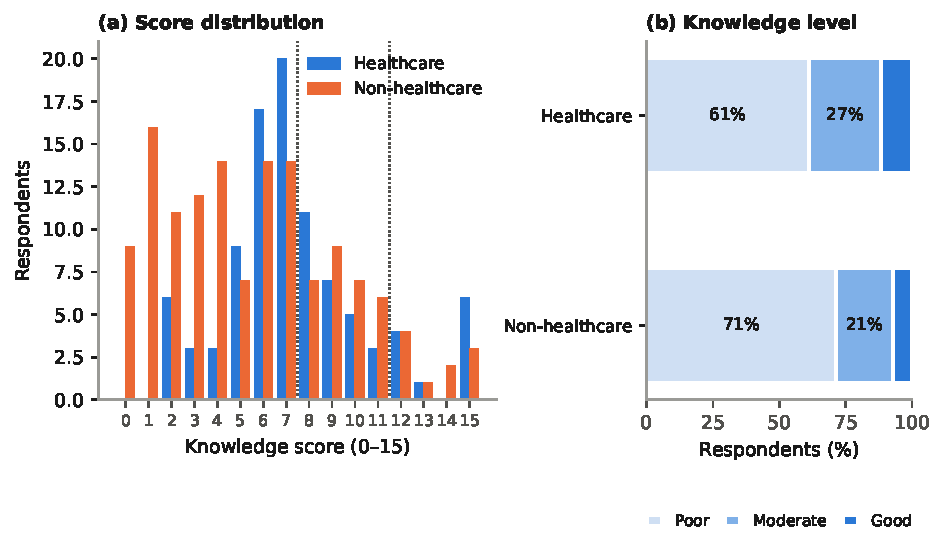
\includegraphics[width=.95\textwidth]{fig_knowledge_dist}
\caption{Distribution of knowledge scores (a) and knowledge levels (b) by academic stream. Dotted lines in (a) mark the cut-offs between poor, moderate and good knowledge.}\label{fig:kdist}
\end{figure}
\FloatBarrier
\begin{table}[htbp]\centering\footnotesize
\caption{Item-wise correct responses on the HPV knowledge statements, overall and by academic stream ($N=231$).}\label{tab:kitems}
\begin{tabularx}{\textwidth}{@{}l >{\raggedright\arraybackslash}X c c c c@{}}\toprule
 & Statement & Overall & Healthcare & Non-healthcare & $p$ \\
 &  & $n$ (\%) & $n$ (\%) & $n$ (\%) &  \\\midrule
K1 & HPV stands for Human Papillomavirus. & 182 (78.8) & 88 (92.6) & 94 (69.1) & $<$0.001 \\
K2 & HPV can infect both males and females. & 114 (49.4) & 48 (50.5) & 66 (48.5) & 0.765 \\
K3 & HPV infection often does not require treatment. & 37 (16.0) & 18 (18.9) & 19 (14.0) & 0.310 \\
K4 & HPV can cause genital warts. & 104 (45.0) & 56 (58.9) & 48 (35.3) & $<$0.001 \\
K5 & HPV can be passed on during sexual intercourse. & 128 (55.4) & 67 (70.5) & 61 (44.9) & $<$0.001 \\
K6 & HPV infection can lead to cervical cancer. & 181 (78.4) & 80 (84.2) & 101 (74.3) & 0.071 \\
K7 & HPV infection causes menstrual problems in women.\textsuperscript{$\dagger$} & 22 (9.5) & 13 (13.7) & 9 (6.6) & 0.072 \\
K8 & Most people infected with HPV show no visible symptoms. & 88 (38.1) & 44 (46.3) & 44 (32.4) & 0.032 \\
K9 & HPV is one of the most common sexually transmitted infections worldwide. & 123 (53.2) & 63 (66.3) & 60 (44.1) & $<$0.001 \\
K10 & An HPV vaccine is currently available. & 121 (52.4) & 55 (57.9) & 66 (48.5) & 0.161 \\
K11 & The HPV vaccine is most effective when given before sexual activity begins. & 70 (30.3) & 33 (34.7) & 37 (27.2) & 0.220 \\
K12 & The HPV vaccine protects against all strains of HPV.\textsuperscript{$\dagger$} & 30 (13.0) & 16 (16.8) & 14 (10.3) & 0.145 \\
K13 & Males can also benefit from the HPV vaccine. & 73 (31.6) & 30 (31.6) & 43 (31.6) & 0.995 \\
K14 & A Pap smear can detect HPV-related abnormal cell changes in the cervix. & 97 (42.0) & 48 (50.5) & 49 (36.0) & 0.028 \\
K15 & Condom use reduces, but does not eliminate, the risk of HPV transmission. & 89 (38.5) & 46 (48.4) & 43 (31.6) & 0.010 \\
\bottomrule\end{tabularx}

\vspace{2pt}\raggedright\scriptsize \textsuperscript{$\dagger$}False statement (correct answer ``False''). All other statements are true. ``Not sure'' and missing responses were scored as incorrect. $p$ from Pearson's $\chi^2$ test, or Fisher's exact test where marked \textsuperscript{F}.
\end{table}

\FloatBarrier
\begin{figure}[htbp]\centering
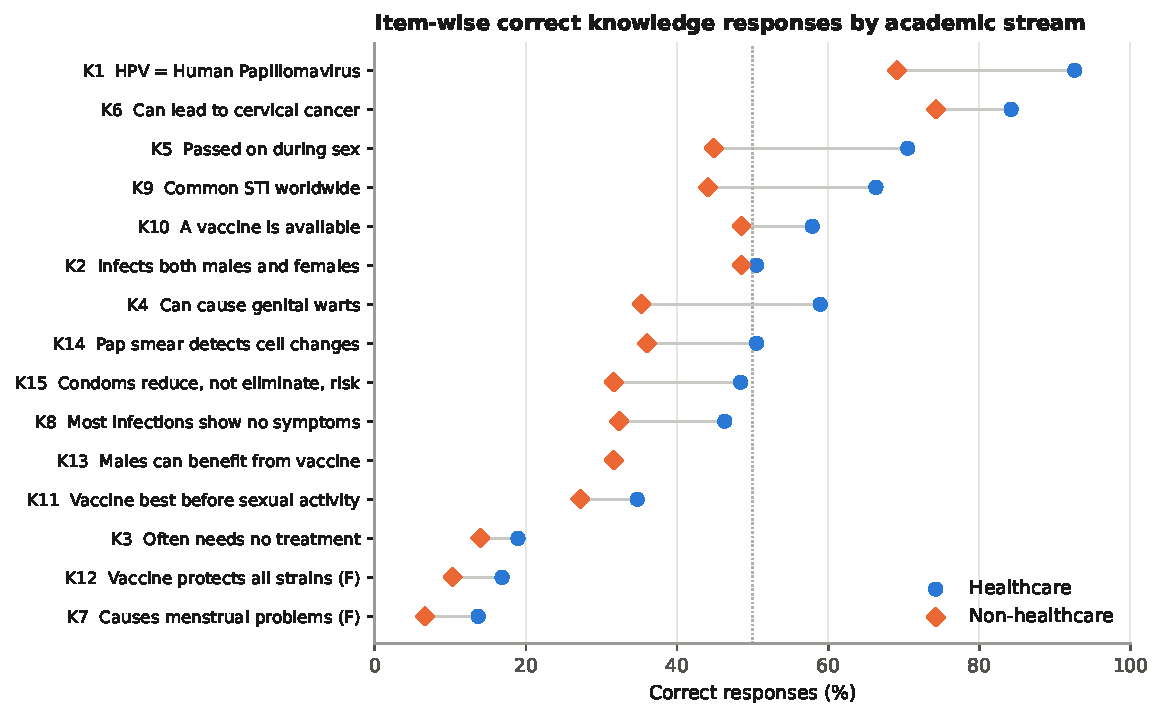
\includegraphics[width=.95\textwidth]{fig_knowledge_items}
\caption{Proportion of correct answers to each knowledge statement by academic stream. (F) marks the two false statements.}\label{fig:kitems}
\end{figure}

\section{Attitudes Towards HPV Prevention and Vaccination}
Attitudes were strongly positive. The mean attitude score was $44.69\pm4.48$ out of 50 (median 45.6, IQR 42.0--48.0). In all, 204 students (88.3\%) had a positive attitude, 26 (11.3\%) a neutral attitude and one (0.4\%) a negative attitude. Healthcare students had a higher mean score than non-healthcare students ($45.56\pm3.91$ against $44.08\pm4.77$; $U=7{,}696.0$, $p=0.013$), but the share with a positive attitude did not differ significantly (91.6\% against 86.0\%, $p=0.22$).

Nearly all students agreed that people should be informed about HPV infection (97.4\%) and about the vaccine (98.7\%), and that women should be informed about its complications (95.6\%). Most agreed that all young women should be vaccinated (91.3\%), that HPV is a serious risk for women (86.8\%) and that they would like to know more about the vaccine (91.2\%). Agreement was lower for making the vaccine mandatory before marriage (75.9\%) and that a Pap smear is necessary for HPV screening (64.8\%), for which 34\% were neutral (Table~\ref{tab:attitudes}, Figure~\ref{fig:att}). A total of 87.0\% agreed that cost and difficulty of access are obstacles in Bangladesh.

Knowledge and attitude scores were positively correlated (Spearman's $\rho=0.316$, $p<0.001$): students who knew more tended to hold more favourable attitudes, although the association was moderate.

\FloatBarrier
\begin{table}[htbp]\centering\footnotesize
\caption{Attitudes towards HPV prevention, screening and vaccination (row percentages; 5-point Likert scale).}\label{tab:attitudes}
\begin{tabularx}{\textwidth}{@{}l >{\raggedright\arraybackslash}X ccccc c@{}}\toprule
 & Statement & SD & D & N & A & SA & Mean $\pm$ SD \\\midrule
A1 & It is necessary to inform people about HPV infection. & 0.9 & 0.0 & 1.8 & 14.9 & 82.5 & 4.78 $\pm$ 0.56 \\
A2 & It is necessary to inform people about the HPV vaccine. & 0.4 & 0.0 & 0.9 & 19.1 & 79.6 & 4.77 $\pm$ 0.50 \\
A3 & It is necessary to inform women about HPV and its complications. & 0.4 & 0.0 & 3.9 & 15.8 & 79.8 & 4.75 $\pm$ 0.57 \\
A4 & All young women should be vaccinated against HPV. & 0.4 & 0.9 & 7.4 & 24.7 & 66.7 & 4.56 $\pm$ 0.71 \\
A5 & The HPV vaccine should be mandatory for women before marriage. & 0.4 & 1.8 & 21.9 & 28.1 & 47.8 & 4.21 $\pm$ 0.88 \\
A6 & I recommend the HPV vaccine to my friends. & 0.4 & 1.3 & 15.2 & 28.1 & 55.0 & 4.36 $\pm$ 0.82 \\
A7 & I would like to know more about the HPV vaccine. & 0.0 & 0.4 & 8.3 & 35.1 & 56.1 & 4.47 $\pm$ 0.67 \\
A8 & HPV infection is a serious risk for women. & 0.9 & 1.8 & 10.6 & 29.5 & 57.3 & 4.41 $\pm$ 0.82 \\
A9 & The high cost and difficulty in accessing the vaccine in Bangladesh are obstacles to vaccination. & 0.0 & 1.3 & 11.7 & 30.9 & 56.1 & 4.42 $\pm$ 0.75 \\
A10 & A Pap smear test is necessary for HPV screening in women. & 0.0 & 1.3 & 33.9 & 30.4 & 34.3 & 3.98 $\pm$ 0.86 \\
\bottomrule\end{tabularx}

\vspace{2pt}\raggedright\scriptsize SD = strongly disagree, D = disagree, N = neutral, A = agree, SA = strongly agree. Item-level non-response was at most four respondents ($\leq$1.7\%).
\end{table}

\FloatBarrier
\begin{figure}[htbp]\centering
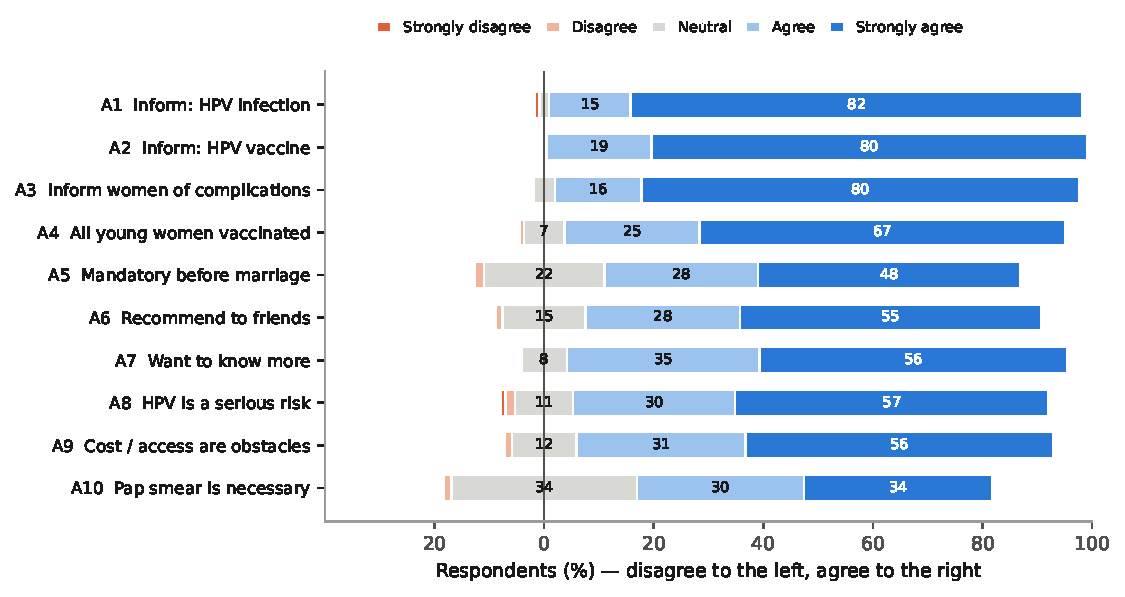
\includegraphics[width=.95\textwidth]{fig_attitudes}
\caption{Responses to the ten attitude statements (percentage of respondents).}\label{fig:att}
\end{figure}

\section{Perceived Barriers to Vaccination}
Lack of awareness of HPV and the vaccine was rated the greatest barrier (mean $3.88\pm1.38$; 69.6\% rated it 4 or 5), followed by the cost of the vaccine (3.79; 68.1\%), lack of a healthcare provider's recommendation (3.73; 65.5\%) and limited availability in health facilities (3.67; 61.6\%) (Table~\ref{tab:barriers}, Figure~\ref{fig:barriers}). Cultural or religious concerns were rated lowest (2.81; 31.3\%).

\begin{table}[htbp]\centering\small
\caption{Perceived barriers to HPV vaccination, ranked by mean rating (1--5 scale; higher = greater barrier).}\label{tab:barriers}
\begin{tabularx}{\textwidth}{@{}c >{\raggedright\arraybackslash}X c c c@{}}\toprule
Rank & Barrier & $n$ & Mean $\pm$ SD & Rated 4--5 (\%) \\\midrule
1 & Lack of awareness about HPV and the vaccine & 230 & 3.88 $\pm$ 1.38 & 69.6 \\
2 & Cost of the vaccine & 229 & 3.79 $\pm$ 1.24 & 68.1 \\
3 & Lack of healthcare-provider recommendation & 229 & 3.73 $\pm$ 1.21 & 65.5 \\
4 & Limited availability in health facilities & 229 & 3.67 $\pm$ 1.26 & 61.6 \\
5 & Fear of side effects & 230 & 3.57 $\pm$ 1.23 & 56.1 \\
6 & Feeling ashamed or judged because of STIs & 230 & 3.28 $\pm$ 1.45 & 49.6 \\
7 & Belief that the vaccine is not necessary & 230 & 3.14 $\pm$ 1.44 & 46.5 \\
8 & Cultural or religious concerns & 227 & 2.81 $\pm$ 1.31 & 31.3 \\
\bottomrule\end{tabularx}\end{table}

\begin{figure}[htbp]\centering
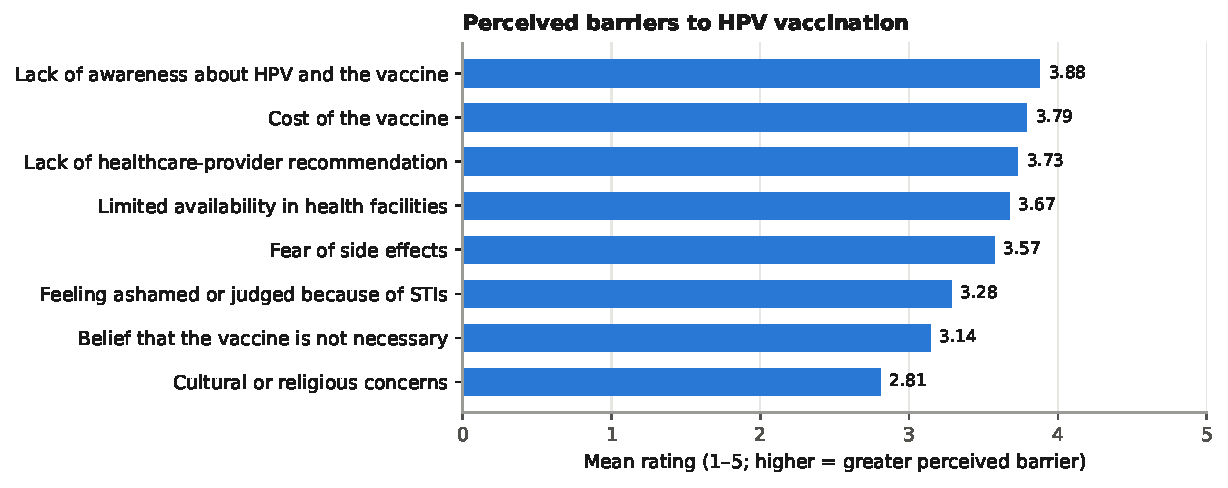
\includegraphics[width=.90\textwidth]{fig_barriers}
\caption{Mean ratings of perceived barriers to HPV vaccination.}\label{fig:barriers}
\end{figure}
\FloatBarrier

\section{Reasons for Not Being Vaccinated and Factors That Would Encourage Vaccination}
Of the 197 students who gave reasons for not being vaccinated, over half (103, 52.3\%) said they did not know about the vaccine. Others cited concern about safety or side effects (38, 19.3\%), unavailability or cost (30, 15.2\%), not thinking they were at risk (29, 14.7\%) and that a doctor had never recommended it (15, 7.6\%). Family or religious opposition was named by one student (Figure~\ref{fig:reasons}a).

When asked what would encourage vaccination, students most often chose a free or subsidised vaccine (106, 45.9\%), a doctor's recommendation (98, 42.4\%) and an educational campaign at university (89, 38.5\%). Availability at a campus health centre (21.6\%), support from family or friends (12.1\%) and knowing someone affected by an HPV-related disease (11.7\%) were chosen less often (Figure~\ref{fig:reasons}b).

Support for educational measures was high (Table~\ref{tab:support}). Among the 200 students who answered the question on provider advice, 164 (82.0\%) said a recommendation from a healthcare provider would definitely or probably increase their likelihood of vaccination. A short video or workshop would definitely or probably improve intention for 191 of 228 students (83.8\%). A total of 205 of 227 (90.3\%) agreed that HPV vaccination should be part of school, college or university health programmes, and 192 of 231 (83.1\%) that HPV education should be compulsory in the curriculum. In the open question, the most frequent suggestions for the government were awareness campaigns, free or subsidised vaccines, and wider availability of the vaccine.

\begin{figure}[htbp]\centering
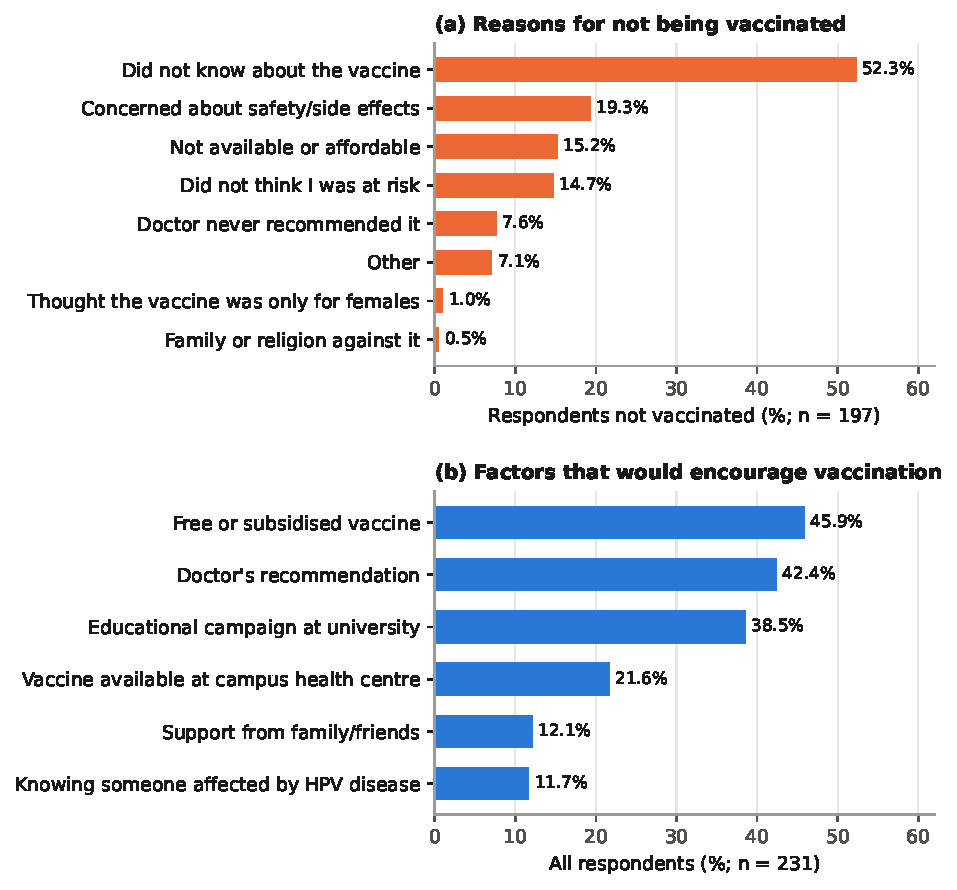
\includegraphics[width=.90\textwidth]{fig_reasons_motivators}
\caption{(a) Reasons for not being vaccinated ($n=197$) and (b) factors that would encourage vaccination ($n=231$). Respondents could select more than one option.}\label{fig:reasons}
\end{figure}
\FloatBarrier
\begin{table}[htbp]\centering\scriptsize
\caption{Views on provider recommendation, educational interventions and institutional policy, $n$ (\%).}\label{tab:support}
\setlength{\tabcolsep}{3pt}
\begin{tabularx}{\textwidth}{@{}>{\raggedright\arraybackslash}X c c c c c c@{}}\toprule
Statement & $n$ & \shortstack{Definitely yes /\\strongly agree} & \shortstack{Probably yes /\\agree} & Not sure / neutral & \shortstack{Probably not /\\disagree} & \shortstack{Definitely not /\\strongly disagree} \\\midrule
A recommendation from a healthcare provider would increase my likelihood of vaccination & 200 & 64 (32.0) & 100 (50.0) & 32 (16.0) & 3 (1.5) & 1 (0.5) \\
A short educational video or workshop would improve my vaccination intention & 228 & 77 (33.8) & 114 (50.0) & 27 (11.8) & 6 (2.6) & 4 (1.8) \\
HPV vaccination should be part of school/college/university health programmes & 227 & 133 (58.6) & 72 (31.7) & 18 (7.9) & 2 (0.9) & 2 (0.9) \\
HPV education should be compulsory in the academic curriculum & 231 & 100 (43.3) & 92 (39.8) & 31 (13.4) & 6 (2.6) & 2 (0.9) \\
\bottomrule\end{tabularx}\end{table}

\FloatBarrier

\section{Factors Associated With Acceptance}
\subsection{Bivariate analysis}
Acceptance did not differ by age, academic stream, parents' education, prior STI education, parental discussion, social taboo or the university's programme (Table~\ref{tab:bivariate}). It was higher among students who had heard of HPV (85.0\% against 63.0\%, $p<0.001$) and among those with a positive attitude (82.7\% against 63.0\%, $p=0.015$). Students who accepted vaccination also had higher knowledge scores (mean 6.55 against 5.09, Mann--Whitney $p=0.011$) and attitude scores (45.03 against 43.31, $p=0.021$). Acceptance rose from 77.4\% among students with poor knowledge to 85.2\% and 90.0\% among those with moderate and good knowledge, but this trend was not statistically significant ($p=0.24$) (Figure~\ref{fig:factors}).

\begin{table}[htbp]\centering\footnotesize
\caption{Association of respondent characteristics with acceptance of HPV vaccination ($n=229$).}\label{tab:bivariate}
\begin{tabularx}{\textwidth}{@{}>{\raggedright\arraybackslash}X c c c c@{}}\toprule
Variable & Total & Accepting & Not accepting & $p$ \\
 & $n$ & $n$ (row \%) & $n$ (row \%) &  \\\midrule
\multicolumn{5}{l}{\textbf{Age (years)}} \\
\quad 18--21 & 60 & 46 (76.7) & 14 (23.3) & 0.526 \\
\quad 22--23 & 104 & 83 (79.8) & 21 (20.2) &  \\
\quad 24 and above & 65 & 55 (84.6) & 10 (15.4) &  \\
\multicolumn{5}{l}{\textbf{Academic stream}} \\
\quad Healthcare & 94 & 75 (79.8) & 19 (20.2) & 0.858 \\
\quad Non-healthcare & 135 & 109 (80.7) & 26 (19.3) &  \\
\multicolumn{5}{l}{\textbf{Parents' education}} \\
\quad University / higher & 171 & 138 (80.7) & 33 (19.3) & 0.773 \\
\quad Below university or unsure & 57 & 45 (78.9) & 12 (21.1) &  \\
\multicolumn{5}{l}{\textbf{Prior STI education}} \\
\quad Yes & 124 & 101 (81.5) & 23 (18.5) & 0.648 \\
\quad No / not sure & 105 & 83 (79.0) & 22 (21.0) &  \\
\multicolumn{5}{l}{\textbf{Had heard of HPV before the survey}} \\
\quad Yes & 180 & 153 (85.0) & 27 (15.0) & $<$0.001 \\
\quad No & 46 & 29 (63.0) & 17 (37.0) &  \\
\multicolumn{5}{l}{\textbf{Parental discussion of HPV}} \\
\quad Yes (brief or detailed) & 79 & 67 (84.8) & 12 (15.2) & 0.218 \\
\quad Never / unsure & 150 & 117 (78.0) & 33 (22.0) &  \\
\multicolumn{5}{l}{\textbf{Discussing HPV is taboo}} \\
\quad Taboo (very much / somewhat) & 157 & 128 (81.5) & 29 (18.5) & 0.475 \\
\quad Not taboo & 71 & 55 (77.5) & 16 (22.5) &  \\
\multicolumn{5}{l}{\textbf{University awareness programme}} \\
\quad Yes & 90 & 76 (84.4) & 14 (15.6) & 0.210 \\
\quad No / not aware & 139 & 108 (77.7) & 31 (22.3) &  \\
\multicolumn{5}{l}{\textbf{Knowledge level}} \\
\quad Poor (0--7) & 155 & 120 (77.4) & 35 (22.6) & 0.244 \\
\quad Moderate (8--11) & 54 & 46 (85.2) & 8 (14.8) &  \\
\quad Good (12--15) & 20 & 18 (90.0) & 2 (10.0) &  \\
\multicolumn{5}{l}{\textbf{Attitude level}} \\
\quad Positive ($\geq$40) & 202 & 167 (82.7) & 35 (17.3) & 0.015 \\
\quad Neutral/negative ($<$40) & 27 & 17 (63.0) & 10 (37.0) &  \\
\multicolumn{5}{l}{\textbf{Continuous variables}} \\
\quad Knowledge score, mean $\pm$ SD & -- & 6.55 $\pm$ 3.59 & 5.09 $\pm$ 3.64 & 0.011\textsuperscript{M} \\
\quad Attitude score, mean $\pm$ SD & -- & 45.03 $\pm$ 4.39 & 43.31 $\pm$ 4.70 & 0.021\textsuperscript{M} \\
\quad Age (years), mean $\pm$ SD & -- & 22.57 $\pm$ 1.53 & 22.24 $\pm$ 1.42 & 0.158\textsuperscript{M} \\
\bottomrule\end{tabularx}

\vspace{2pt}\raggedright\scriptsize $p$ from Pearson's $\chi^2$ test (Fisher's exact test where marked \textsuperscript{F}; Mann--Whitney $U$ test where marked \textsuperscript{M}). Totals vary slightly because of missing responses.
\end{table}

\FloatBarrier
\begin{figure}[htbp]\centering
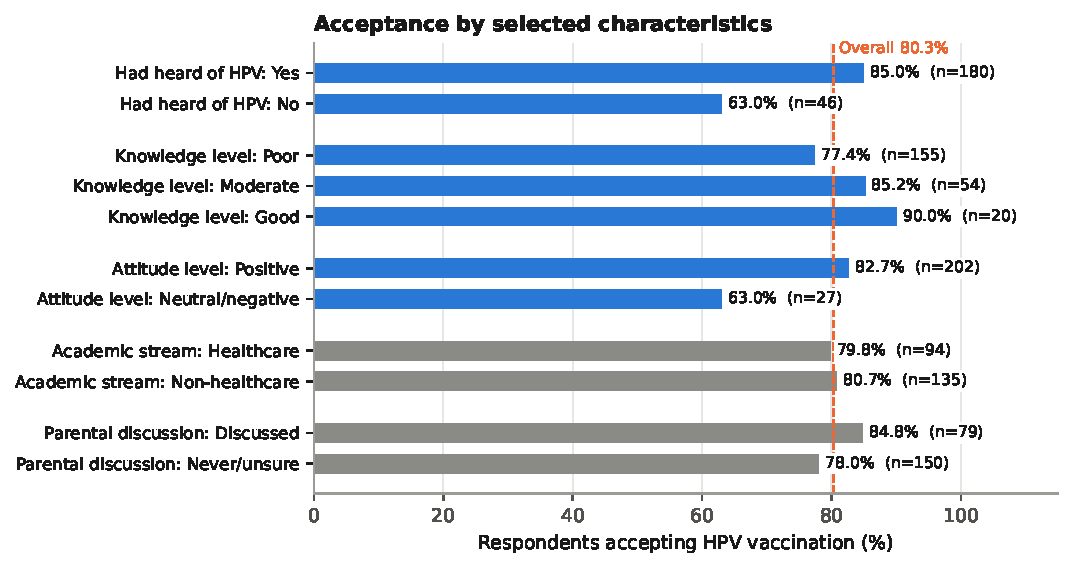
\includegraphics[width=.95\textwidth]{fig_acceptance_factors}
\caption{Percentage of students accepting HPV vaccination by selected characteristics. The dashed line shows the overall level (80.3\%).}\label{fig:factors}
\end{figure}

\subsection{Multivariable analysis}
In Model 1, having heard of HPV was the only variable independently associated with acceptance (AOR 3.14, 95\% CI 1.38--7.16, $p=0.006$). The knowledge score was not significant after adjustment (AOR 1.09 per point, 95\% CI 0.97--1.21, $p=0.138$) (Table~\ref{tab:logistic}, Figure~\ref{fig:forest}). When attitude score was added in Model 2, having heard of HPV remained associated with higher odds of acceptance (AOR 3.31, 95\% CI 1.44--7.61, $p=0.005$), and each additional attitude point raised the odds by 8\% (AOR 1.08, 95\% CI 1.00--1.17, $p=0.048$). The models were modest in explanatory power (Nagelkerke $R^2$ = 0.107 and 0.132; AUC = 0.67 and 0.70). The same pattern was seen in the sensitivity analysis restricted to unvaccinated or unsure students (Appendix~C).

\FloatBarrier
\begin{table}[htbp]\centering\footnotesize
\caption{Logistic regression of factors associated with acceptance of HPV vaccination.}\label{tab:logistic}
\setlength{\tabcolsep}{3.5pt}
\begin{tabularx}{\textwidth}{@{}>{\raggedright\arraybackslash}X cc cc cc@{}}\toprule
 & \multicolumn{2}{c}{Unadjusted} & \multicolumn{2}{c}{Model 1} & \multicolumn{2}{c}{Model 2} \\
\cmidrule(lr){2-3}\cmidrule(lr){4-5}\cmidrule(lr){6-7}
Variable & OR (95\% CI) & $p$ & AOR (95\% CI) & $p$ & AOR (95\% CI) & $p$ \\\midrule
Age (per year) & 1.15 (0.93--1.43) & 0.203 & 1.16 (0.91--1.47) & 0.236 & 1.20 (0.94--1.53) & 0.150 \\
Healthcare stream (vs non-healthcare) & 0.94 (0.49--1.82) & 0.858 & 0.67 (0.30--1.49) & 0.327 & 0.64 (0.28--1.43) & 0.271 \\
Parent with university education (vs not) & 1.12 (0.53--2.34) & 0.773 & 1.06 (0.49--2.32) & 0.879 & 1.07 (0.49--2.35) & 0.863 \\
Prior STI education (vs none/unsure) & 1.16 (0.61--2.24) & 0.648 & 1.02 (0.49--2.09) & 0.966 & 1.06 (0.51--2.20) & 0.866 \\
Had heard of HPV (vs not) & 3.32 (1.61--6.86) & 0.001 & 3.14 (1.38--7.16) & 0.006 & 3.31 (1.44--7.61) & 0.005 \\
Parents discussed HPV (vs never/unsure) & 1.57 (0.76--3.25) & 0.220 & 1.16 (0.53--2.53) & 0.717 & 1.16 (0.52--2.56) & 0.715 \\
Knowledge score (per point) & 1.13 (1.02--1.24) & 0.017 & 1.09 (0.97--1.21) & 0.138 & 1.06 (0.95--1.18) & 0.322 \\
Attitude score (per point) & 1.08 (1.01--1.16) & 0.026 & -- & -- & 1.08 (1.00--1.17) & 0.048 \\
\midrule
$n$ analysed (accepting) & \multicolumn{2}{c}{--} & \multicolumn{2}{c}{225 (181)} & \multicolumn{2}{c}{225 (181)} \\
Nagelkerke $R^2$ & \multicolumn{2}{c}{--} & \multicolumn{2}{c}{0.107} & \multicolumn{2}{c}{0.132} \\
AUC & \multicolumn{2}{c}{--} & \multicolumn{2}{c}{0.673} & \multicolumn{2}{c}{0.703} \\
\bottomrule\end{tabularx}

\vspace{2pt}\raggedright\scriptsize OR = odds ratio; AOR = adjusted odds ratio; CI = confidence interval. Outcome: accepting (1) vs not accepting (0). Model 1 includes socio-demographic variables, prior awareness and knowledge score; Model 2 additionally adjusts for attitude score. Respondents with missing data on any model variable were excluded.
\end{table}

\FloatBarrier
\begin{figure}[htbp]\centering
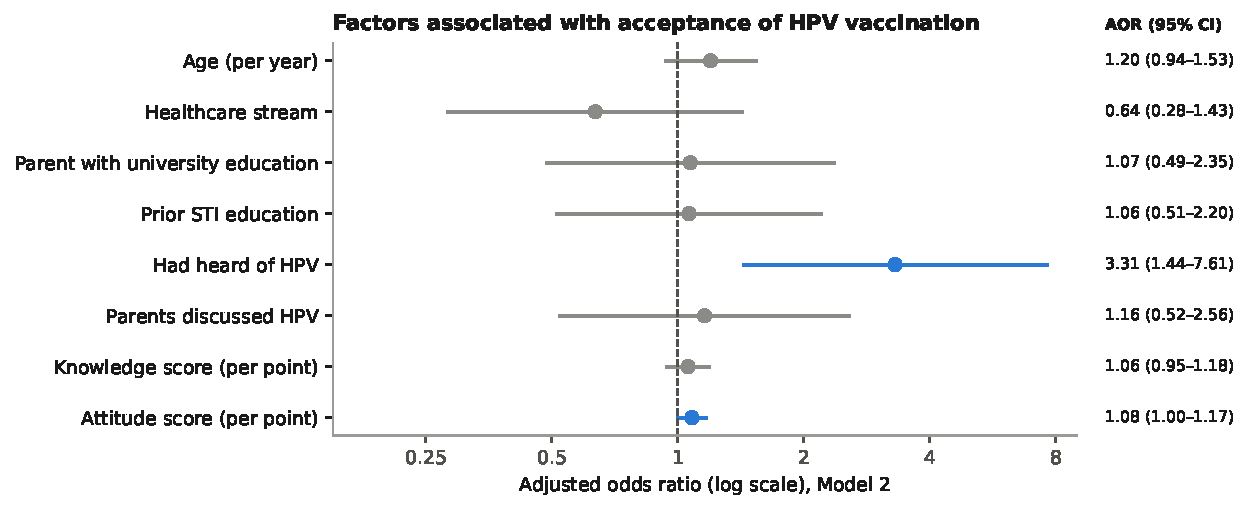
\includegraphics[width=.95\textwidth]{fig_forest}
\caption{Adjusted odds ratios for acceptance of HPV vaccination (Model 2, $n=225$). Blue marks $p<0.05$.}\label{fig:forest}
\end{figure}
\FloatBarrier
